\chapter{Recap particle physics}
\section{Units}
In general natural units are used: $\hbar = \mathrm c = 1$
\begin{compactitem}
    \item[$\ra$] energy, mass and momentum: $\qty[ E]$
    \item[$\ra$] length and time: $\qty[ E] ^{-1}$
    \item[$\ra$] cross section: $\qty[ E] ^{-2}$
\end{compactitem}
\begin{example}
\begin{align*}
    \hbar \mr c \approx \SI{200}{\mega\eV\femto\meter} \,\hat =\, 1 \longrightarrow \SI{1}{\femto \meter} \,\hat\approx\, \SI{5}{\per\giga\eV}\\
    \hbar = \SI{6.6 e-25}{\giga \eV \second} \,\hat = 1\, \longrightarrow \SI{1}{\per \giga \eV} \,\hat \approx\, \SI{6.6e-25}{\second}
\end{align*}
\end{example}

Additionally: use the Heaviside units for electromagnetic processes
\begin{compactitem}[$\rightarrow$]
    \item take the Coulomb force between to charged particles (with charge e)
    \begin{align*}
        F_\mathrm{C} = \frac{\mathrm e^2}{4 \pi \upvarepsilon_0 r^2} \qquad \overset{\upvarepsilon_0 \equiv 1}{\longrightarrow} \frac{\mathrm e^2}{4 \pi r^2}
    \end{align*}
    \item remember that $\upvarepsilon_0 \upmu_0 = \mathrm c^{-2}$, which leads to $\upmu_0 = 1$
\end{compactitem}
In total we use in particle physics:
\begin{align}
    \bm{\boxed{\hbar = \mr c = \upvarepsilon_0 = \upmu_0 = 1}}
\end{align}





\section{Relativistic kinematics}
We will use four vector notation, i.e.
\begin{align}
    \fvec A = \qty( A^0, \vec A) \longrightarrow A^\mu & & \text{contravariant}\\
    \qty( A^0, -\vec A) \longrightarrow A_\mu & & \text{covariant.}
\end{align}
\paragraph{Lorentz trafos}
Remember that the Lorentz transformation $\uul \Lambda$:
\begin{align}
    A^\mu \mapsto A'^\mu = \tensor{\Lambda}{^\mu_\nu}A^\nu
\end{align}
The transformation along the $z$-axis  is a Lorentz-boost
\begin{align}
    \tensor{\Lambda}{^\mu_\nu} \ra \uul \Lambda = \mqty(\gamma & 0 &  0 &- \nicefrac \gamma \beta \\ 0 & 1 & 0 & 0 \\ 0 & 0 & 1 & 0 \\ - \nicefrac \gamma \beta & 0 & 0 & \gamma) \qquad \text{ with } \beta = \frac vc, \ \gamma = \frac{1}{\sqrt{1-\beta^2}}\,.
\end{align}
The Lorentz transformation is a \tb{unitary} transformation: ''rotation in 4-space``
\paragraph{Momentum four vector}
\begin{align}
    x^\mu \ra \fvec x = \qty( t, \vec x), \qquad E = \gamma m \mr c^2 = \gamma m, \qquad \vec p = \gamma m \vec v = \gamma m \vec \beta
\end{align}
So it is easy to see that the momentum vector $\vec p$ is measured in units of energy. Thus we may choose the following four vector as momentum four vector (and indeed it is)
\begin{align}
    p^\mu \ra \fvec p = \qty( E, \vec p ), \qquad \Ra E^2 = \vec p^2 +m^2\,.
\end{align}
\paragraph{Basic invariant} under Lorentz transformation is the scalar product
\begin{align}
    \fvec A \cdot \fvec B = A^\mu B_\mu = \tensor{g}{_\mu_\nu} A^\mu B^\nu = A_\mu B^\mu = A^0B^0 - \vec A \vec B\\
    \text{with } \tensor{g}{_\mu_\nu} = \tensor{g}{^\mu^\nu} = \mat{1 & 0 & 0 & 0 \\ 0 & -1 & 0 & 0 \\ 0 & 0 & -1 & 0 \\ 0 & 0 & 0 & -1} \text{ as metric tensor.} \nonumber
\end{align}
\begin{example}
    scalar product of four momentum $\fvec p$
    \begin{align}
        p^2 = p^\mu p_\mu = E^2 - \vec p^2 = m^2\,,
    \end{align}
    since $E^2 = \vec p^2 +m^2$. Therefore the (rest) mass of the particle is the same in all frames of reference.
\end{example}
\begin{example}
    total energy $\sqrt s$ of particle collision
    \begin{center}
        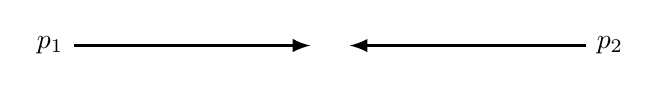
\begin{tikzpicture}
            \draw[very thick, -latex] (0,0) node [left] {$\fvec p_1$} -- (3,0);
            \draw[very thick, latex-] (3.5,0) -- (6.5,0) node [right] {$\fvec p_2$};
        \end{tikzpicture}
    \end{center}
    \begin{align}
        s \defi \qty( \fvec p_1 + \fvec p_2)^2 = \qty( \fvec p_1 + \fvec p_2 )^\mu \qty( \fvec p_1 + \fvec p_2 )_\mu 
    \end{align}
    is Lorentz invariant since it is a scalar product. Hence it is the same in all reference frames.
\end{example}
\paragraph{Four vector derivatives}
\begin{align}
    \pa_\mu = \pdv{x^\mu} \ra \qty( \pa_t, \vec \grad )
\end{align}
transforms like a covariant vector. Whereas
\begin{align}
    \pa^\mu = \pdv{x_\mu} \ra \qty(t, - \vec \grad)
\end{align}
transforms like a controvariant vector. The ''scalar product`` of these two is the d'Alembert operator
\begin{align}
    \Box \defi \pa_\mu\pa^\mu = \pa_t^2 - \Lap\,,
\end{align}
\begin{compactitem}
    \item[with] the Laplace operator $\Lap = \vec \grad^2$.
\end{compactitem}

\section{Elementary particles}
\paragraph{Fermions (spin $\nicefrac 12$)} Lepton sector:
\begin{align}
    \mqty(\upnu_\mr{e} \\\mr e^- ), \quad \mqty(\upnu_\upmu \\ \upmu^-),\quad \mqty(\upnu_\uptau \\ \uptau^-) \qquad \text{with charges } \mqty{Q = 0 \\ Q= -\mr e}
\end{align}
They come with a certain mass hierarchy $m_\mr{e} < m_\upmu < m_\uptau$ and the assumption in the standard model that $m_\upnu = 0$ regardless of the neutrino flavour. However we know $m_\upnu >0$ but very small.

Quark sector:
\begin{align}
    \mqty(u \\ d), \quad \mqty(c \\ s), \quad \mqty( t \\ b) \qquad \text{with charges } \mqty{Q = \frac 23 \mr e \\ Q = - \frac 13 \mr e}
\end{align}
Free particles are bounded states with $qq'q''$ as baryons and $q\bar q$ as mesons. Additionally, only colour-neutral particle states are observed.

Both sectors come with the respective 6 anti-particles.

\paragraph{Bosons (spin $1$)} exchange particles of interactions
\begin{compactitem}
    \item[$\upgamma$:] em. interaction, $m=0$, $Q=0$ couples to electric charge
    \item[$Z^0$:] weak interaction, $m = \SI{91}{\giga\eV}$, $Q=0$, couples to weak charge
    \item[$W^\pm$:] weak interaction, $m = \SI{80}{\giga\eV}$, $Q = \pm \mr e$, couples to weak charge
    \item[$g$:] strong interaction, $m=0$, $Q=0$\\
    8 gluons in total, carry colour charge\\
    couple to quarks and to one another (''self-coupling``)
\end{compactitem}

\paragraph{Scalar (spin $0$)}
\begin{compactitem}
    \item[$H^0$:] Higgs boson, brings mass to $Z^0$, $W^\pm$ (''spontaneous symmetry breaking``)\\
    $m = \SI{125}{\giga\eV}$
\end{compactitem}

\section{Feynman diagrams}
These give pictorial representations of particle reactions. Perturbative expansion of scattering ''in a potential`` into leading order and higher order terms, if necessary.
\begin{example}
    electromagnetic scattering (leading order)
    \begin{multicols}{2}
        \begin{center}
            \begin{tikzpicture}
                \begin{feynman}
                \vertex (a1);
                \vertex [below right = 2cm of a1] (b1);
                \vertex [above right = 2cm of b1] (a2);
                \vertex [below = 2cm of b1] (c1);
                \vertex [below left = 2cm of c1] (d1);
                \vertex [below right = 2cm of c1] (d2);
                \vertex [below left = 0.5cm of d1] (z1);
                \vertex [right = 1.6cm of z1] (z2);
                \vertex [below right = 0.5cm of d2] (z4);
                \vertex [left = 1.6cm of z4] (z3);
                \vertex [below = 2.2cm of c1] (y1) {particles};
                \diagram*{
                (a1) -- [fermion, edge label = $\mr e^-$, momentum' = $\fvec p_1$] (b1) -- [fermion, edge label = $\mr e^-$, momentum' = $\fvec p_1'$] (a2),
                (b1) -- [photon, edge label' = $\upgamma$, momentum = $\fvec q$] (c1),
                (d1) -- [fermion, edge label' = $\upmu^-$, momentum = $\fvec p_2$] (c1) -- [fermion, edge label' = $\upmu^-$, momentum = $\fvec p_2'$] (d2);
                };
                \draw[decoration={brace}, decorate] (z2.south) -- node[below] {incoming} (z1.south west);
                \draw[decoration={brace}, decorate] (z4.south east) -- node[below] {outgoing} (z3.south);
                \end{feynman}
            \end{tikzpicture}
        \end{center}
        \begin{compactitem}
            \item[with] $\fvec q$: 4-momentum transfer
        \end{compactitem}
        We will describe this in $\fvec q^2$ (which is Lorentz invariant)
        \begin{align}
            \fvec q^2 = \qty(\fvec p_1 - \fvec p_1')^2 \neq 0
        \end{align}
        The inequity to zero means that it is off mass-shell\\
        $\Ra$ virtual particle because it carries to much/less energy
    \end{multicols}
    
    Next question to ask is: What is the \tb{transition amplitude}?
    \begin{multicols}{2}
        \begin{center}
            \begin{tikzpicture}
                \begin{feynman}
                    \vertex (b1);
                    \vertex [above left  = 1cm of b1] (a1) {$\mr e^-$};
                    \vertex [above right = 1cm of b1] (a2) {$\mr e^-$};
                    \vertex [below = 1cm of b1] (c1);
                    \vertex [below left  = 1cm of c1] (d1) {$\upmu^-$};
                    \vertex [below right = 1cm of c1] (d2) {$\upmu^-$};
                    \diagram*{
                        (a1) -- [fermion] (b1) -- [fermion] (a2),
                        (b1) -- [scalar, momentum = {$\fvec q, M$}] (c1),
                        (d1) -- [fermion] (c1) -- [fermion] (d2);
                    };
                \end{feynman}
            \end{tikzpicture}
        \end{center}
    \begin{align}
        amplitude \propto g_1 \frac{1}{\fvec q^2 - M^2} g_2
    \end{align}
    \begin{compactitem}
        \item[with] $g_{1,2}$: coupling strength between fermion and exchange particle
        \item[] $\nicefrac{1}{\fvec q^2-M^2}$: boson propagator for exchange particle of mass $M$
    \end{compactitem}
    \end{multicols}
    Here the electromagnetic and the weak interaction contribute, i.e.
    \begin{align*}
        \feynmandiagram[vertical'= b to d, baseline = -2cm]{
        a [particle = $\mr e^-$] -- [fermion] b -- [fermion] c [particle = $\mr e^-$];
        b -- [photon, edge label = $\upgamma$] d;
        e [particle = $\upmu^-$]-- [anti fermion] d -- [anti fermion] f [particle = $\upmu^-$];
        };
        + 
        \feynmandiagram[vertical'= b to d, baseline = -2cm]{
        a [particle = $\mr e^-$] -- [fermion] b -- [fermion] c [particle = $\mr e^-$];
        b -- [scalar, edge label = $Z^0$] d;
        e [particle = $\upmu^-$]-- [anti fermion] d -- [anti fermion] f [particle = $\upmu^-$];
        };
        = e \frac{1}{\fvec q^2}e + g_1 \frac{1}{\fvec q^2 - M_Z^2} g_2
    \end{align*}
    Last question: What is the \tb{cross section}?\\
    It is proportional to the transition probability
    \begin{align}
        \sigma \propto W, \qquad W \propto \qty| amplitude_1 + amplitude_2 |^2 \propto \frac{\mr e^4}{\fvec q^4}
    \end{align}
    The factor $\nicefrac{1}{\fvec q^4}$ leads to a rapid decrease of the cross section as momentum transfer increases. In the centre of mass system this can be depicted as:
    \begin{center}
			\tdplotsetmaincoords{60}{130}
			\begin{tikzpicture}[tdplot_main_coords]
            \coordinate (O) at (0,0,0);
            \tdplotsetcoord{P}{3.5}{30}{90};
            \tdplotsetcoord{P1}{5}{40}{90};
            \node at (P1) [xshift = 1em, yshift = 1em] {$\fvec p_1' = \qty(E_1', \vec p_1')$};
            \draw[-latex] (0,-3.25,0) node [above left] {$\fvec p_1$} node [below left] {$\mr e^-$} -- (0,-.25,0);
            \draw[latex-] (0,.25,0) -- (0,3.25,0) node [above right] {$\fvec p_2$} node [below right] {$\upmu^-$};
            \draw[-latex] (O) -- (P);
            \tdplotsetthetaplanecoords{90};
            \tdplotdrawarc[tdplot_rotated_coords]{(0,0,0)}{1}{30}{90}{anchor = north, xshift = -.5em, yshift = .5em}{$\theta$};
            \tdplotdrawarc[tdplot_rotated_coords, -latex, myblue]{(0,0,0)}{2}{30}{0}{anchor = south east, xshift = -1em}{incr. $\fvec q^2$};
            %
            \tdplotsetthetaplanecoords{80};
            \tdplotdrawarc[tdplot_rotated_coords]{(0,0,0)}{3.5}{20}{40}{anchor=south west}{};
            \tdplotsetthetaplanecoords{100};
            \tdplotdrawarc[tdplot_rotated_coords]{(0,0,0)}{3.5}{20}{40}{anchor=south west}{};
            \foreach \i in {-10,-9,...,9}
                \draw (xyz spherical cs:radius=3.5, latitude=50, longitude=\i) -- (xyz spherical cs:radius=3.5, latitude=50, longitude=\i+1);
            \foreach \i in {-10,-9,...,9}
                \draw (xyz spherical cs:radius=3.5, latitude=70, longitude=\i) -- (xyz spherical cs:radius=3.5, latitude=70, longitude=\i+1);
        \end{tikzpicture}
    \end{center}
    Then $ W \propto \nicefrac{1}{\fvec q^4}$ $\longrightarrow$ mostly forward scattering $\qty(\theta \approx \SI{0}{\degree})$.\\
    cf.: Rutherford scattering
    \begin{align}
        \dv{\sigma}{\Omega} \propto \frac{1}{\sin[4](\nicefrac{\theta}{2})}\,.
    \end{align}
\end{example}

The above example sketches only the leading order terms. Thus the question arises how one would calculate the full scattering amplitude?
\begin{align}
    \feynmandiagram[vertical = b to d, baseline = -1.5cm, small]{
        a [particle = $\mr e^-$] -- [fermion] b -- [fermion] c [particle = $\mr e^-$],
        b -- [scalar, opacity = 0] d,
        e [particle = $\upmu^-$]-- [fermion] d -- [fermion] f [particle = $\upmu^-$],
    };
    =
    & \underbrace{
    \feynmandiagram[vertical = b to d, baseline = -1.5cm, small]{
        a -- [fermion] b -- [fermion] c,
        b -- [photon] d,
        e -- [fermion] d -- [fermion] f,
    };
    }_\text{1\textsuperscript{st} order}
    +
    \underbrace{
    \feynmandiagram[vertical = b to g, baseline = -1.45cm, small]{
        a -- [anti fermion] b -- [anti fermion] c -- [anti fermion] d,
        b -- [photon] g,
        c -- [photon] f,
        e -- [fermion] f -- [fermion] g -- [fermion] h,
    };
    + 
    \feynmandiagram[vertical = c to g, baseline = -1.75cm, small]{
        a -- [fermion] b -- [fermion] c -- [fermion] d -- [fermion] e,
        b -- [photon, half left] d,
        c -- [photon] g,
        f -- [anti fermion] g -- [anti fermion] h,
    };
    + 
    \feynmandiagram[vertical = b to d, baseline = -2.1cm, small]{
        a -- [anti fermion] b -- [anti fermion] c,
        b -- [photon] d -- [fermion, half left] e -- [photon] g,
        d -- [anti fermion, half right] e,
        f -- [anti fermion] g -- [anti fermion] h,
    };
    }_\text{2\textsuperscript{nd} order}
    \nonumber \\
    & +
    \underbrace{
    \feynmandiagram[vertical = b1 to e3, baseline = -1.45cm, small]{
        a -- [anti fermion] b1 -- [anti fermion] b2 -- [anti fermion] b3 -- [anti fermion] c,
        b1 -- [photon] e3,
        b2 -- [photon] e2,
        b3 -- [photon] e1,
        d -- [fermion] e1 -- [fermion] e2 -- [fermion] e3 -- [fermion] f,
    };
    + \dots}_\text{3\textsuperscript{rd} order}
    + \dots
    \nonumber \\
    full\ amplitude = & \underset{\propto \mr e^2 \propto \alpha}{\text{leading order}} + \underset{\propto \mr e^4 \propto \alpha^2}{\text{2\textsuperscript{nd} order}} + \underset{\propto \mr e^6 \propto \alpha^3}{\text{3\textsuperscript{rd} order}}
\end{align}
\begin{compactitem}
    \item[with] $\displaystyle \alpha = \frac{\mr e^2}{4 \pi \hbar \mr c \upvarepsilon_0} = \frac{1}{137}$
\end{compactitem}
Thus in QED it is sufficient to only calculate the first order. It is sufficient to understand the basics of the process (cross section, angular distributions). For comparison to precision measurements sometimes more than 100 diagrams have to calculated.
